\subsubsection{Submódulo Mediciones}
Correspondiente a las pruebas de hardware, en primera instancia se probo el submódulo de mediciones el cual consiste en verificar que el caudalimetro este midiendo de manera adecuada y este arrojando la salida deseada, en este caso se espera una señal digital que tenga un voltaje de 5 VPP.
\\
Para la prueba se utilizo un osciloscopio y se introdujeron por el caudalimetro 500 ml de agua, el caudalimetro se energizo con 5v. Los resultados obtenidos en el osciloscopio se muestran en la figura \ref{fig:senial_caudal}.
\begin{figure}[H]
	\centering
	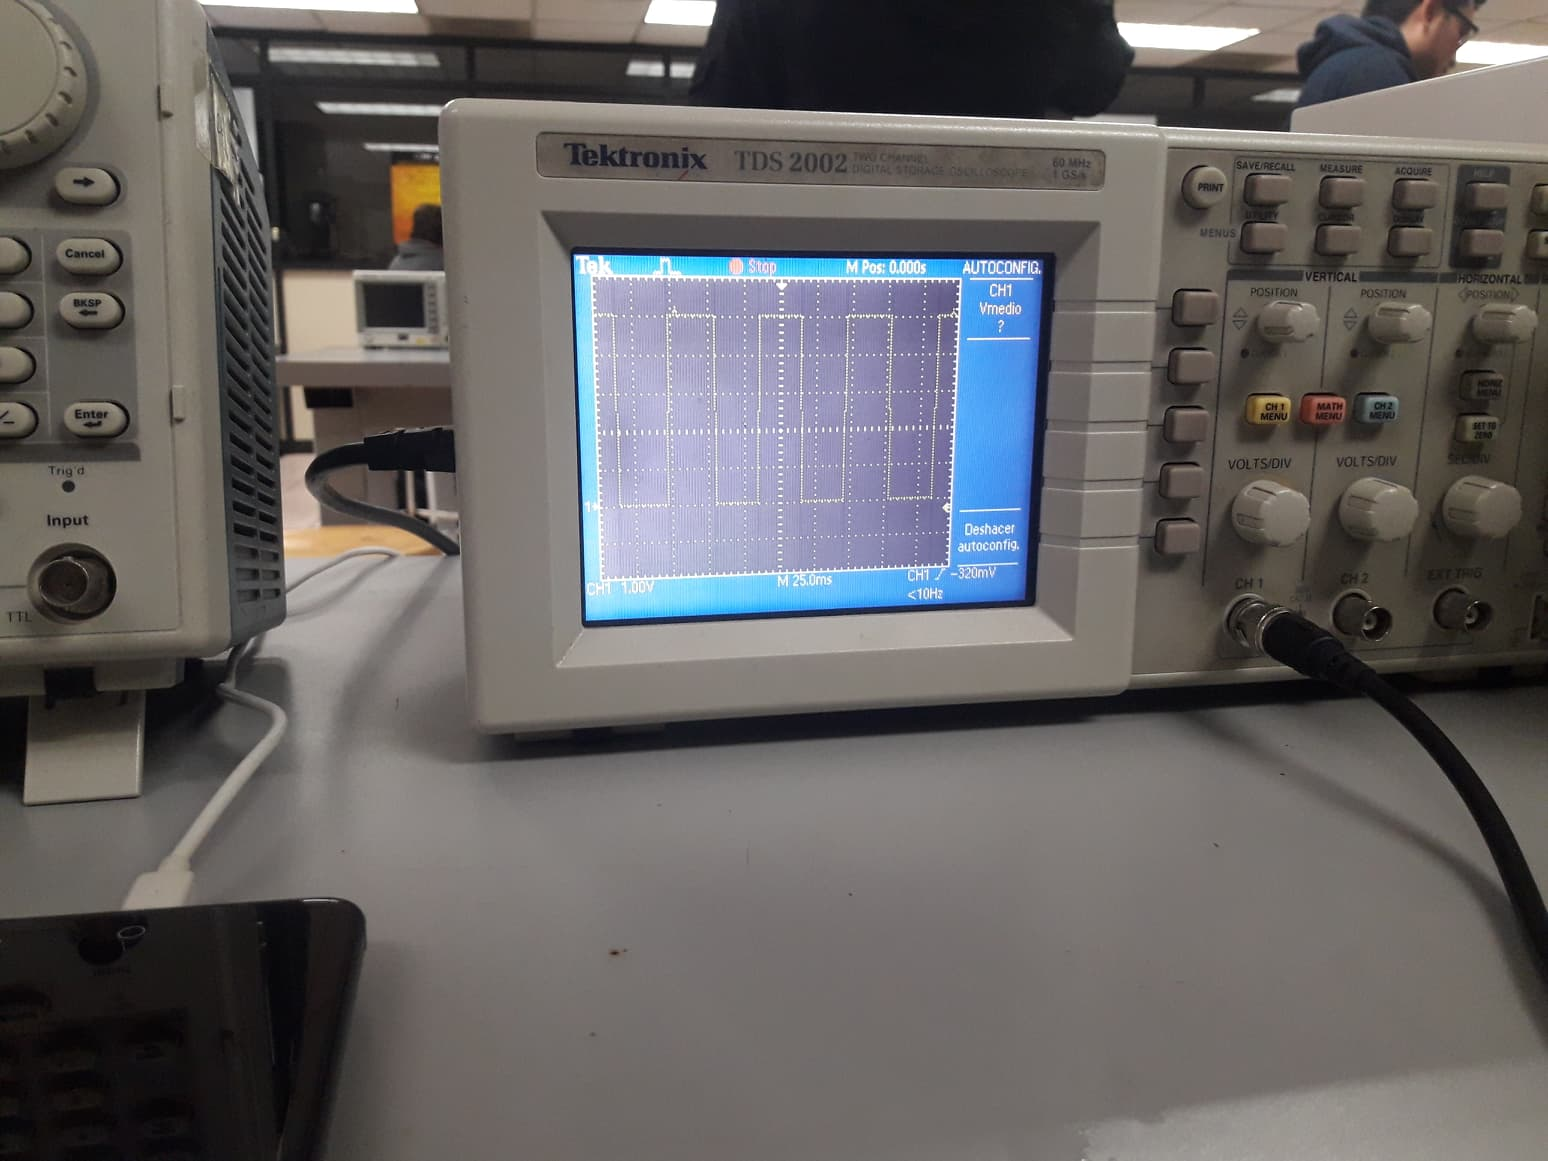
\includegraphics[width=1\textwidth]{Capitulo6/unitarias/hardware/img/senial}
	\caption{Señal obtenida en el osciloscopio}
	\label{fig:senial_caudal}
\end{figure}
Como se puede observar en la figura anterior la señal obtenida por el caudalimetro es digital por lo cual esto puede ser tratado directamente por el microcontrolador sin la necesidad de acondicionar la señal.
\\
En la imagen \ref{fig:senial_caudal_anexo} se muestra una segunda prueba de la salida del caudalimetro, esto con el fin de corroborar el correcto funcionamiento del dispositivo.
\begin{figure}[H]
	\centering
	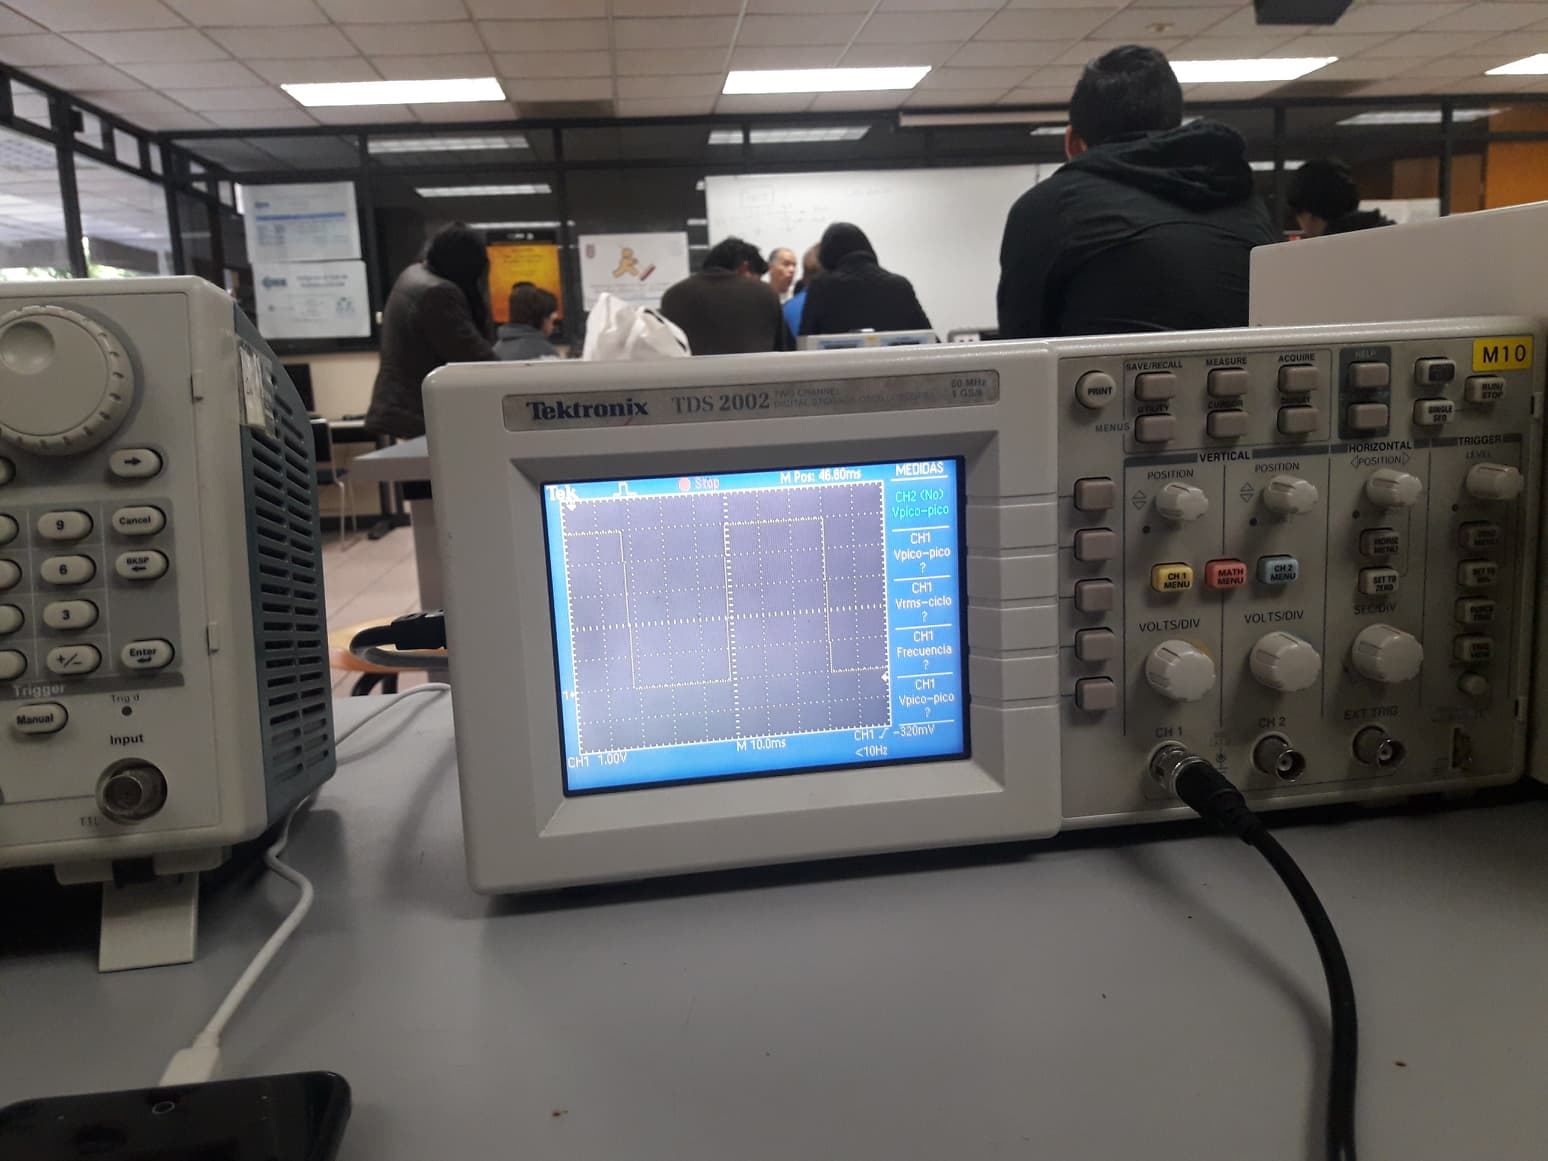
\includegraphics[width=1\textwidth]{Capitulo6/unitarias/hardware/img/senial_2}
	\caption{Señal obtenida en el osciloscopio(Prueba 2)}
	\label{fig:senial_caudal_anexo}
\end{figure}